
\documentclass[12pt]{article}
\setlength\parindent{0pt}
\usepackage{fullpage}
\usepackage[margin=0.5in]{geometry}
\usepackage{amsmath}
\usepackage{graphicx}
\setlength{\parskip}{4mm}
\def\LL{\left\langle}   % left angle bracket
\def\RR{\right\rangle}  % right angle bracket
\def\LP{\left(}         % left parenthesis
\def\RP{\right)}        % right parenthesis
\def\LB{\left\{}        % left curly bracket
\def\RB{\right\}}       % right curly bracket
\def\PAR#1#2{ {{\partial #1}\over{\partial #2}} }
\def\PARTWO#1#2{ {{\partial^2 #1}\over{\partial #2}^2} }
\def\PARTWOMIX#1#2#3{ {{\partial^2 #1}\over{\partial #2 \partial #3}} }
\newcommand{\BE}{\begin{displaymath}}
\newcommand{\EE}{\end{displaymath}}
\newcommand{\BNE}{\begin{equation}}
\newcommand{\ENE}{\end{equation}}
\newcommand{\BEA}{\begin{eqnarray}}
\newcommand{\EEA}{\nonumber\end{eqnarray}}
\newcommand{\EL}{\nonumber\\}
\newcommand{\la}[1]{\label{#1}}
\newcommand{\ie}{{\em i.e.\ }}
\newcommand{\eg}{{\em e.\,g.\ }}
\newcommand{\cf}{cf.\ }
\newcommand{\etc}{etc.\ }
\newcommand{\Tr}{{\rm tr}}
\newcommand{\etal}{{\it et al.}}
\newcommand{\OL}[1]{\overline{#1}\ } % overline
\newcommand{\OLL}[1]{\overline{\overline{#1}}\ } % double overline
\newcommand{\OON}{\frac{1}{N}} % "one over N"
\newcommand{\OOX}[1]{\frac{1}{#1}} % "one over X"



\begin{document}
\pagenumbering{gobble}
\Large
\centerline{\sc{Homework 7}}

\normalsize
\centerline{\sc{Due before class on Tuesday, April 13}}

\begin{enumerate}

\item Suppose that two small spacecraft, each with a mass of 2000 kg, are drifting next to each other. One of them has an astronaut on board; with her equipment, she has a mass of 200 kg. 

	Both craft are moving in the $x-$direction at a velocity of $\vec v_i = (0.5~\rm m/\rm s, 0)$. An astronaut wants to travel from one to the other. She pushes off of one spacecraft and jumps onto the other craft; as she floats through the air, she travels in the $y-$direction with a velocity of $\vec v_a = (0, 1~\rm m/\rm s)$. Note that when she moves through the air, she is moving {\it only} in the y-direction.


		\begin{enumerate}
			\item What will the velocity of the first spacecraft be after she jumps off of it? {\it (Velocity is a vector; you can give its components.)}

			
			\item What will the velocity of the second spacecraft be after she lands on it?
			

			\item Explain in words why the $y-$components of their final velocities are {\it almost} equal and opposite, but are not quite the same magnitude.

			\item Explain in words why the $x-$components of their final velocities are {\it almost} equal. 
		\end{enumerate}

\bigskip

\item Two people, Alice and Bob, are sitting on sleds on a frozen lake; one of them carries a heavy puck with them. They are separated by a distance $d$. The people plus their sleds each have a mass $m_1$; the puck has a mass $m_2$.

	Suppose that the coefficient of kinetic friction between the objects and the lake is $\mu_k$.

	If Alice slides the puck to Bob at a velocity $v_0$, and Bob picks it up, how far will Bob drift before coming to rest?

		{\bf Hint 1:} The ``third kinematics relation'' $v_f^2 - v_0^2 = 2a\Delta x$ that you derived back in February will be very useful here, since you are never interested in the {\it time} these motions take, but care about relating the change in velocity to the distance traveled and the acceleration.

		{\bf Hint 2:} There are multiple things that happen here. Conservation of momentum will help you understand some of them, but not others. First, draw four cartoons, and identify which method you can use to understand how to connect each cartoon to the next:

		\begin{itemize}
	\item Right after Alice slides the puck to Bob
	\item Right before Bob picks up the puck
	\item Right after Bob picks up the puck
	\item When Bob comes to rest
		\end{itemize}



\bigskip\bigskip
\newpage
	\item Consider the demo from class on Thursday: a person stands on a platform that is free to rotate. They are initially not rotating. You can approximate the person as a cylinder (with radius $r_p$ and mass $m_p$) in calculating their moment of inertia.
	
		Someone hands the person a horizontal wheel of radius $r_w$ of mass $m_w$ that is rotating rapidly (clockwise) around its vertical axis at angular velocity $\omega_0$.

		\begin{enumerate}
			\item When the person turns the bicycle wheel over (so it is rotating counterclockwise as seen from above rather than clockwise, for instance), how quickly and in which direction will they begin to rotate?

			\item In class, the bicycle wheel was filled with concrete; its mass was likely around $m_w = 5$ kg. Estimate $r_p$ and $m_p$ for an average person, and estimate $r_w$. Is your result for the final angular velocity of the person reasonable? {\it (The moment of inertia of a thin ring, like the wheel, is $MR^2$; the moment of inertia of a cylinder is $\frac{1}{2}MR^2$.)}
		\end{enumerate}

\bigskip\bigskip

	\item We return to our astronaut using a jet pack to maneuver in space.
	
	\begin{minipage}{0.6\textwidth}
		It consists of a backpack worn by the astronaut with a horizontal bar sticking out from their hips with four thrusters on the ends of the bar. These thrusters are capable of emitting puffs
of gas at 300 m/s; each one is located 60 cm off to the side.

	\end{minipage}
		\begin{minipage}{0.3\textwidth}
			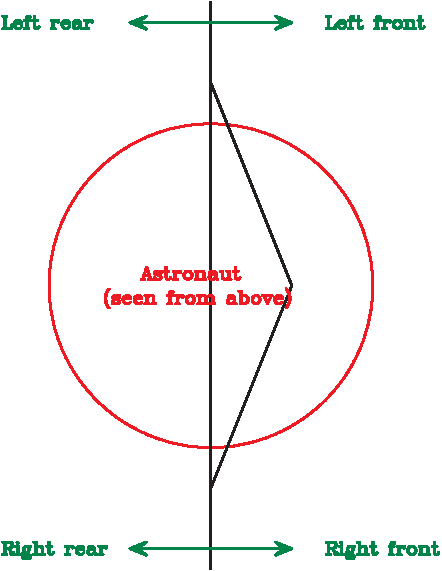
\includegraphics[width=0.9\textwidth]{jetpack-crop.pdf}
		\end{minipage}

		An astronaut wearing this design of jetpack is floating in space, conducting a repair on a satellite, when someone throws them a 20 kg tool at 1 m/s. However, they throw it to the side; the astronaut must reach 
				their arm one meter to the left to catch the tool. 

				\begin{enumerate}
					\item Explain why the astronaut begins to rotate counterclockwise and why they begin to move backwards after they catch the tool.
					

					
					\item What will the astronaut's angular velocity and what will their velocity be after they catch it?

					\item If the astronaut has a mass of 200 kg, and their mass distribution can be approximated by a cylinder of radius 20 cm, how fast will they be rotating?
					

					
					\item They would like to use this jetpack to stop themselves from rotating. Which thrusters should they fire, and how much gas should they release from each one? {\it (Remember that the thrusters are 60 cm from the center.)} There are multiple correct answers here!
					

					
					\item What will their velocity be after this maneuver? What should the astronaut do if they want to reduce their velocity back to zero?
				\end{enumerate}




\end{enumerate}
\end{document}
